\documentclass{ime-beamer}
\usepackage[portuges]{babel}
\usepackage[utf8]{inputenc}
\usepackage{graphicx}
\usepackage{listings}			% Para usar \lstinputlisting e incluir código
\usepackage{color}
\usepackage{multicol}

\definecolor{dkgreen}{rgb}{0,0.6,0}
\definecolor{gray}{rgb}{0.5,0.5,0.5}
\definecolor{mauve}{rgb}{0.58,0,0.82}

\title[Torre de Hanoi]{%
  Torre de Hanoi
}
\author[Luis Helder\and Victor Bramigk \and Jan Segre]{%
  Luis Helder\\
  Victor Bramigk\\
  Jan Segre\\
}

% as imagens ficam nesse diretório
\graphicspath{{img/}}

\begin{document}

\frame{\maketitle}

\frame{%
  \frametitle{Roteiro}
  \tableofcontents
}

%\frame{%
%  \frametitle{Robótica}
%  \begin{block}{}
%  \end{block}
%}

\section{Introdução}
\frame{%
  \frametitle{Problema}
  \begin{figure}
    \centering
    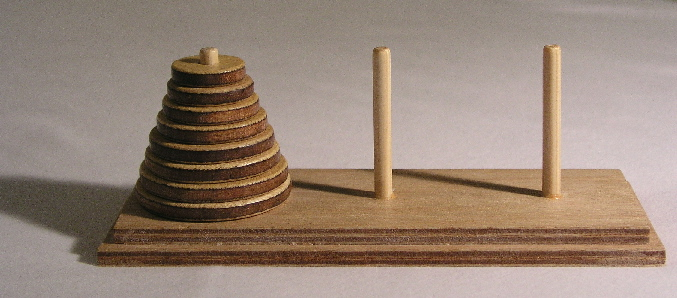
\includegraphics[width= 0.8\linewidth]{Tower_of_Hanoi}
    \caption{Torre de Hanoi}
  \end{figure}
% From:
% "Tower of Hanoi". Licensed under CC BY-SA 3.0 via Wikimedia Commons - 
%  http://commons.wikimedia.org/wiki/File:Tower_of_Hanoi.jpeg#/media/File:Tower_of_Hanoi.jpeg
}

\section{Modelagem}
\frame{%
  \frametitle{Modelagem}
  \begin{block}{}
    \begin{itemize}
      \item Cinemática Inversa
      \item Coleta das posições dos objetos
      \item Solução da Torre de Hanoi
      \item Controle do Robô
    \end{itemize}
  \end{block}
}

\subsection{Cinemática Inversa}
\frame{%
  \frametitle{Cinemática Inversa}
  \begin{block}{}
    \begin{itemize}
      \item Solução Numérica através do Método de Newton
      \item Modelagem inicial no Octave
      \item Tradução para C++ para possibilitar envio via serial
      \item Problema com restrições do braço
      \item Solução: resolver analiticamente
    \end{itemize}
  \end{block}
}

\subsection{Coleta das posições dos objetos}
\frame{%
  \frametitle{Coleta das posições dos objetor}
  \begin{block}{}
    \begin{itemize}
      \item OpenCV: \textit{Open Source Computer Vision}
      \item Separação da imagem através de cores
      \item Cálculo do centroide de cada conjunto de pixels
      \item Conversão das coordenadas da câmera para
            as coordenadas da torre e do braço
    \end{itemize}
  \end{block}
}

\subsection{Solução da Torre de Hanoi}
\frame{%
  \frametitle{Solução da Torre de Hanoi}
  \begin{block}{}
    \begin{itemize}
      \item Identificação da torre
      \item Conversão das coordernadas
      \item Cálculo da order dos discos a serem movidos
      \item Cinemática inversa
      \item Envio dos comando ao braço via serial
    \end{itemize}
  \end{block}
}

\frame{%
  \frametitle{Solução da Torre de Hanoi}
  \begin{block}{}
    Simulação
  \end{block}
}

\subsection{Controle do Robô}
\frame{%
  \frametitle{Controle do Robô}
  \begin{figure}
    \centering
    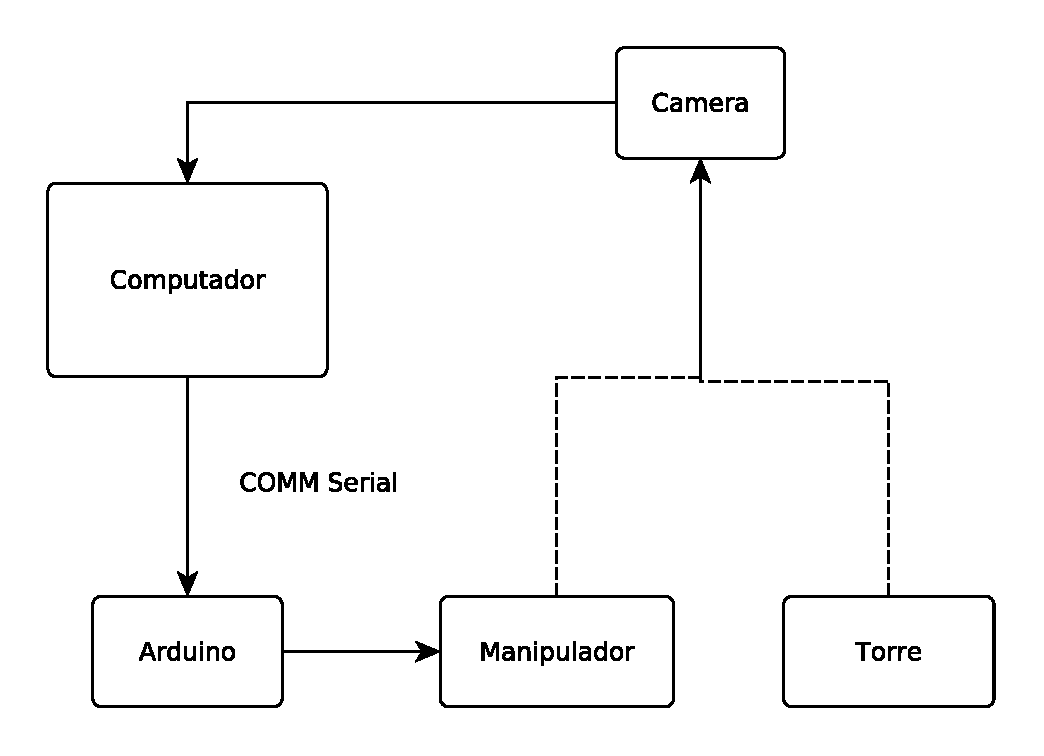
\includegraphics[width= 0.5\linewidth]{sistema}
    \caption{Diagrama dos componentes do sistema}
  \end{figure}
}

\section{Dificuldades}
\frame{%
  \frametitle{Dificuldades}
  \begin{block}{}
    \begin{itemize}
      \item Precisão dos motores: 1 grau
      \item Incorporação das restrições dos motores
            junto com o método numérico
    \end{itemize}
  \end{block}
} 

\section{Resultados}
\frame{%
  \frametitle{Resultados}
  \begin{block}{}
    \begin{itemize}
      \item Cinemática Inversa
      \item Simulador
      \item Solução da Torre de Hanoi
      \item Identificador de marcos através de imagens
    \end{itemize}
  \end{block}
}

\end{document}
% vim: tw=80 et ts=2 sw=2 sts=2
